\section{\textbf{Classification de caract\'eristiques locales}}

Dans la suite du TP, nous avons choisi de traiter le probl\`eme \textit{Visages} de la base d'images Essex. L'objectif g\'en\'eral est d'isoler les pixels de la peau du reste de l'image, afin de localiser pr\'ecis\'ement le visage sur l'image \`a partir d'une classification de caract\'eristiques locales.

\subsection{\textbf{Classification bayésienne des pixels}}

%TODO: Reducri cantidad de texto, dejar lo verdaderamente importante de esta seccion

La classification bay\'esienne des pixels consiste \`a attribuer \`a chaque pixel de l'image une classe en fonction d'un vecteur d'observation construit \`a partir de caract\'eristiques locales, typiquement les composantes de couleur ou d'autres descripteurs calcul\'es autour du pixel. Dans le cadre de ce TP, l'id\'ee est de mod\'eliser probabilistiquement chaque classe \`a partir d'exemples annot\'es, puis de d\'ecider pour chaque pixel la classe la plus probable au sens bay\'esien.

Conform\'ement \`a la section 3.1 du sujet, on commence par visualiser les composantes pertinentes avec le script \texttt{Display\_Components.py}, puis on s\'electionne des exemples d'apprentissage pour apprendre un mod\`ele avec \texttt{Bayes\_Model\_Training.py}. L'apprentissage est supervis\'e : l'utilisateur fournit, \`a l'aide de la souris et du clavier, des r\'egions d'exemples appartenant \`a la classe positive et \`a la classe n\'egative. Le mod\`ele estim\'e permet ensuite de classer l'ensemble des pixels de l'image selon la probabilit\'e associ\'ee \`a chaque classe.

Dans notre probl\`eme \textit{Visages}, cette approche revient \`a distinguer principalement les pixels de peau des pixels de non-peau. La classe positive correspond donc aux zones du visage que l'on souhaite extraire, tandis que la classe n\'egative regroupe l'arri\`ere-plan, les cheveux, les v\^etements et les autres parties de l'image. L'objectif est d'obtenir une segmentation suffisamment pr\'ecise pour localiser le visage de mani\`ere fiable.

\subsubsection{\textbf{Analyse des couleurs}}

Afin d'\'evaluer la s\'eparabilit\'e visuelle entre la peau et le non-peau avant 
l'apprentissage, nous avons ex\'ecut\'e le script \texttt{Display\_Components.py} 
sur l'image \texttt{img/Essex\_Faces/94/asamma.19.jpg}, issue du jeu de donn\'ees 
des visages. Les sorties ont \'et\'e sauvegard\'ees dans 
\texttt{outputs/components/asamma.19/rgb}, 
\texttt{outputs/components/asamma.19/hsv} et 
\texttt{outputs/components/asamma.19/ycrcb} (voir Figure \ref{fig:face_components_spaces}). 
Les fichiers \texttt{original.png} pr\'esents dans chacun de ces r\'epertoires correspondent \`a la m\^eme image source, tandis que les figures de synth\`ese permettent de comparer les d\'ecompositions dans les trois espaces colorim\'etriques.

\begin{figure*}[htbp]
\centering
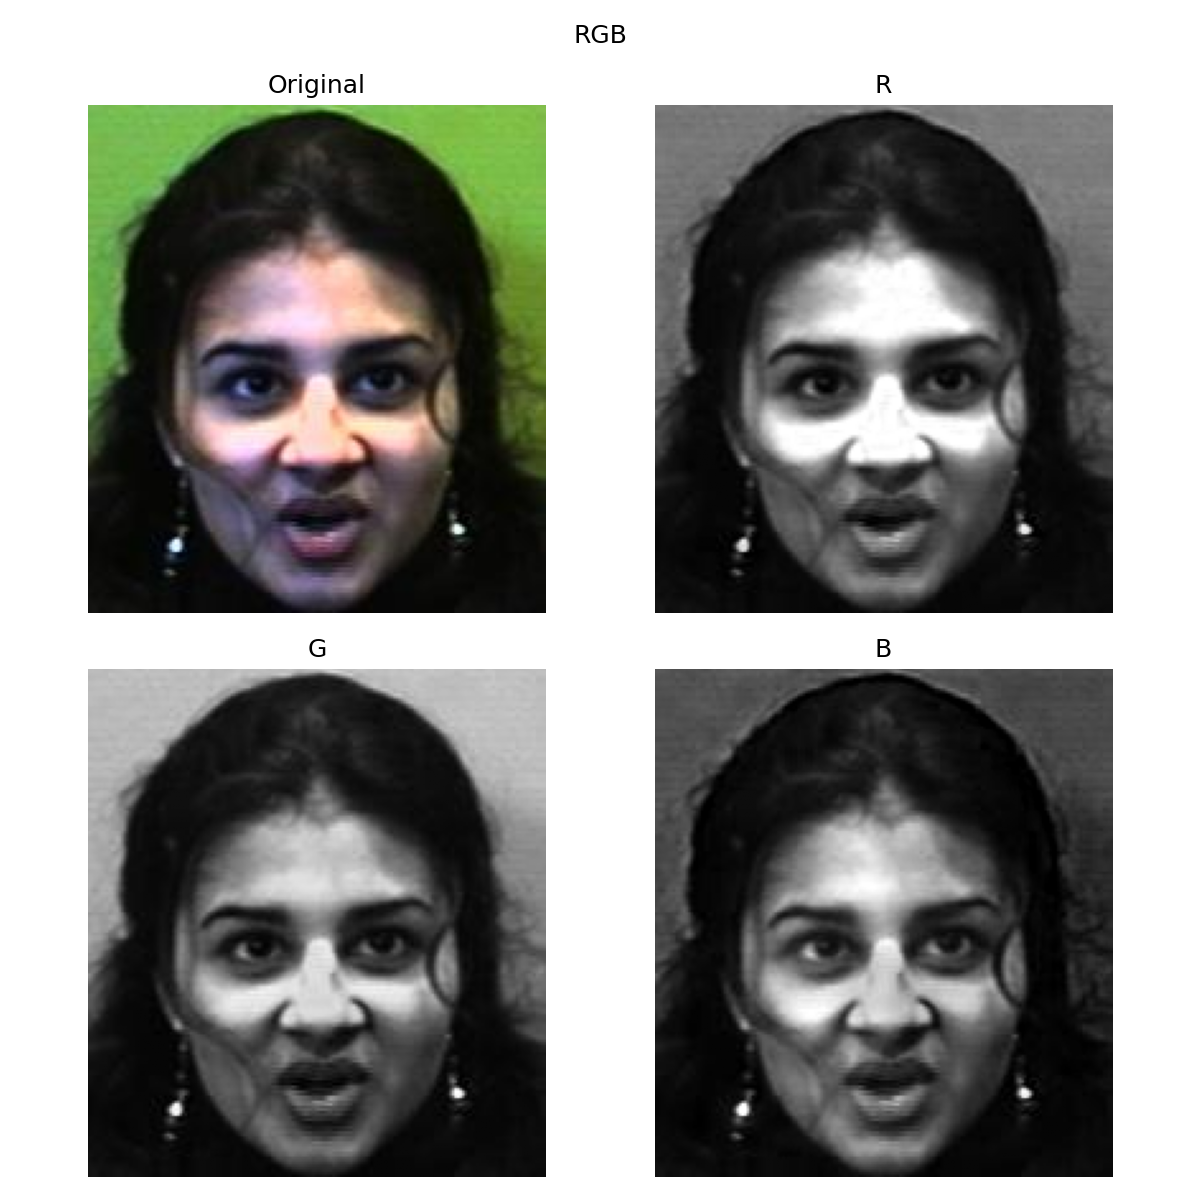
\includegraphics[width=0.32\textwidth]{../../outputs/components/asamma.19/rgb/figure.png}\hfill
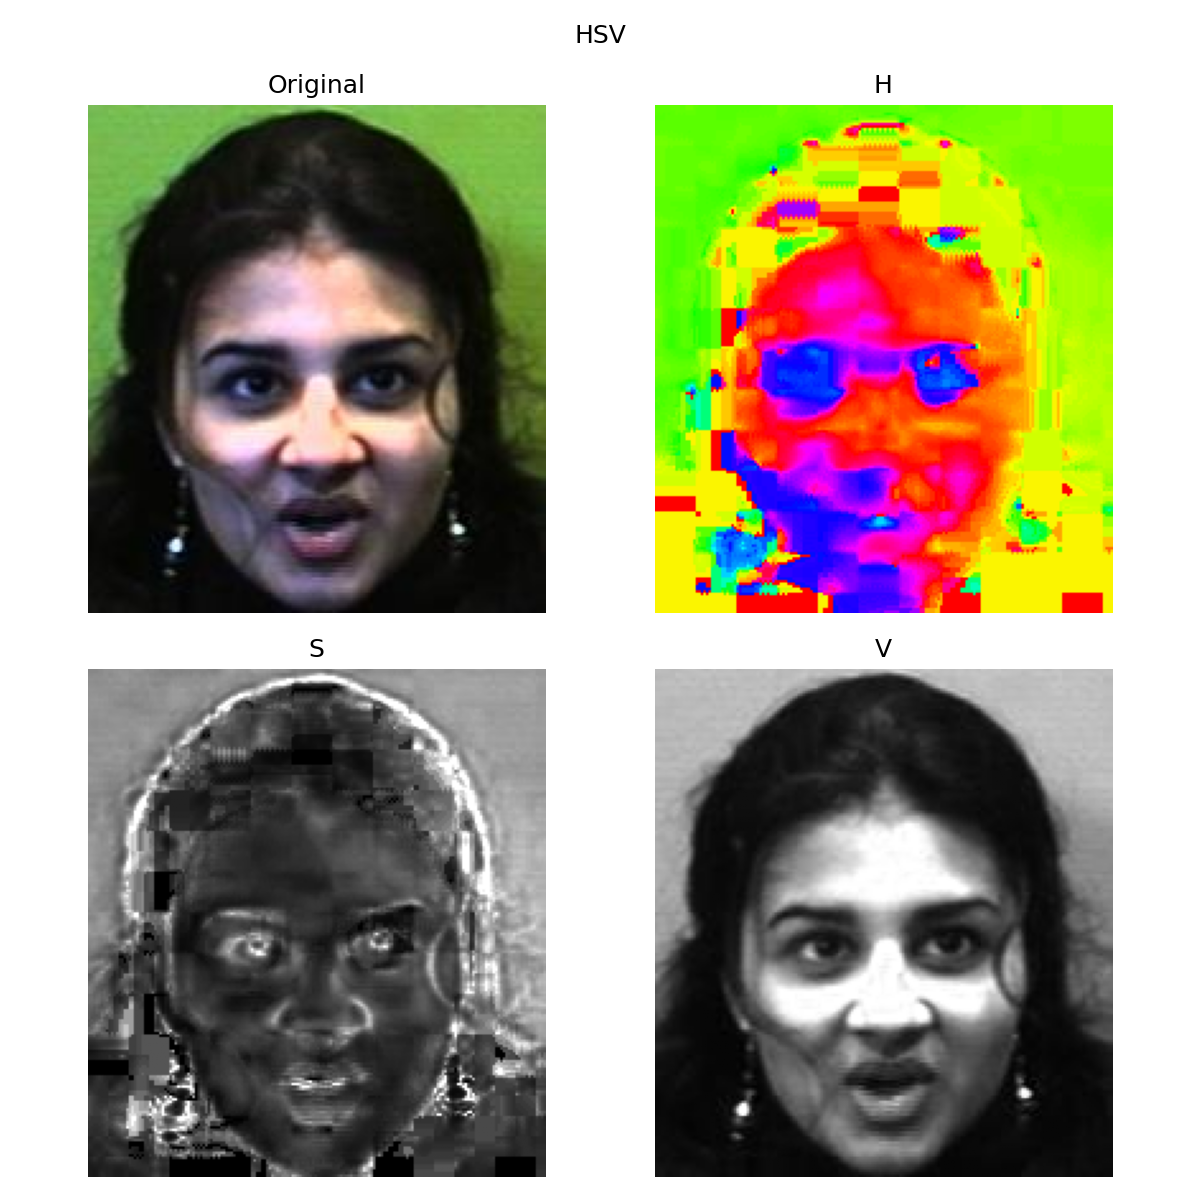
\includegraphics[width=0.32\textwidth]{../../outputs/components/asamma.19/hsv/figure.png}\hfill
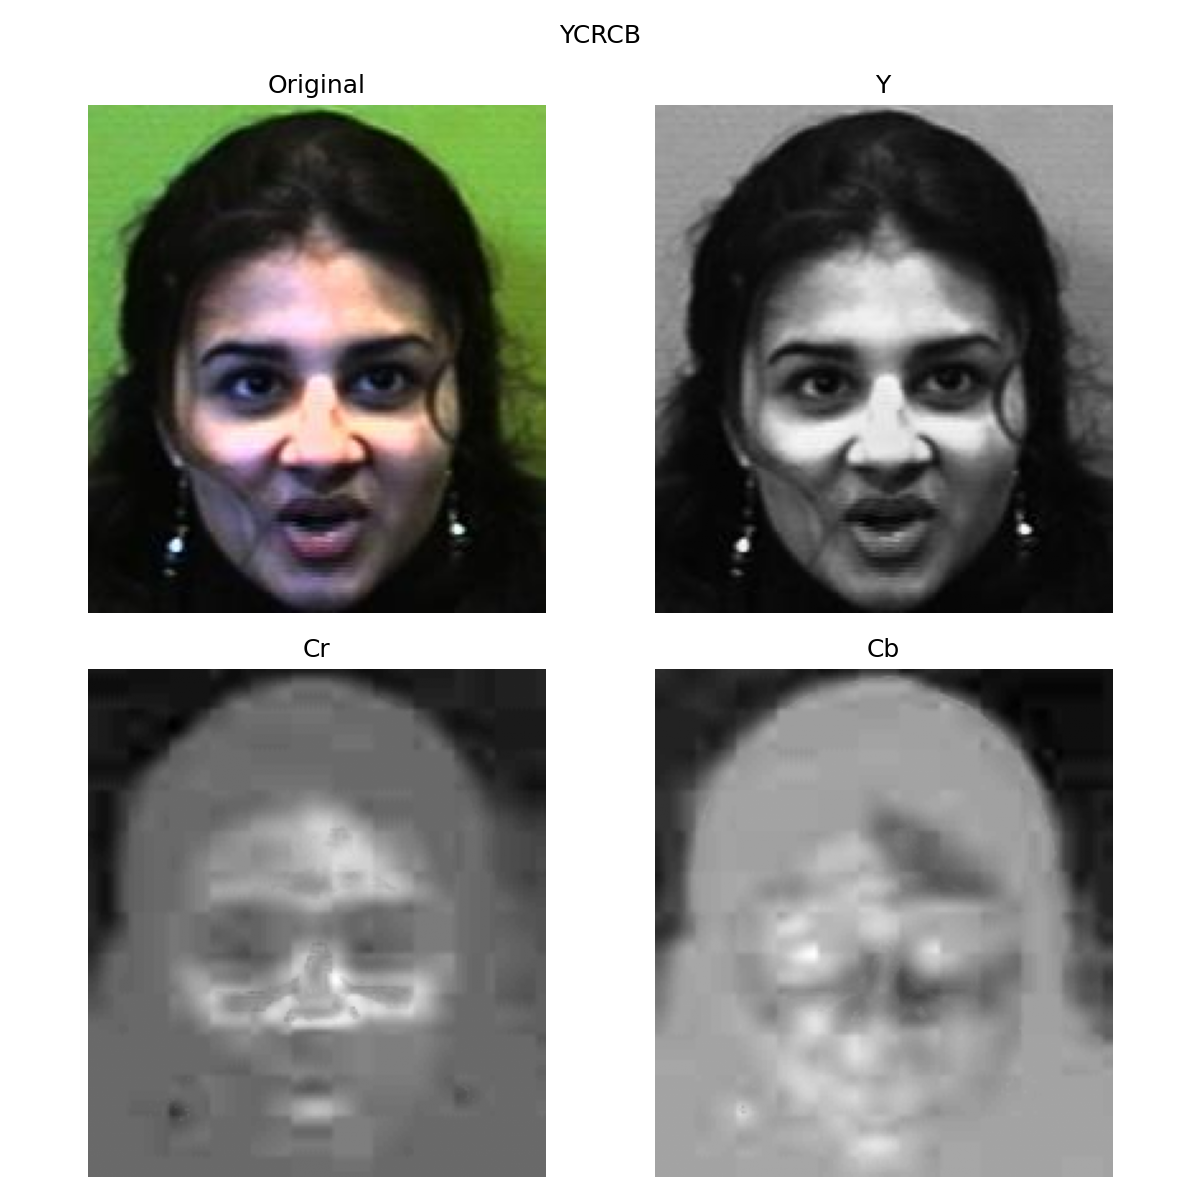
\includegraphics[width=0.32\textwidth]{../../outputs/components/asamma.19/ycrcb/figure.png}
\caption{D\'ecompositions RGB, HSV et YCrCb de l'image \texttt{asamma.19.jpg}, g\'en\'er\'ees avec \texttt{Display\_Components.py}. Chaque figure contient l'image originale ainsi que les trois composantes de l'espace consid\'er\'e.}
\label{fig:face_components_spaces}
\end{figure*}

L'espace RGB fournit une lecture directe des intensit\'es rouge, verte et bleue, mais il m\'elange l'information de chrominance et l'information d'illumination. Sur cette image, le fond vert est relativement bien distingu\'e dans le canal \(G\), et la peau ressort davantage dans le canal \(R\). N\'eanmoins, les variations d'\'eclairage sur le front, le nez et les joues restent fortement pr\'esentes dans les trois canaux, ce qui risque de rendre le mod\`ele moins stable d'une image \`a l'autre.

L'espace HSV s\'epare partiellement la couleur de la luminance via les composantes \(H\), \(S\) et \(V\). La composante \(V\) conserve la structure g\'en\'erale du visage, mais la composante \(H\) appara\^it ici plus instable et bruit\'ee, notamment dans les zones de faible saturation ou pr\`es des transitions abruptes. La composante \(S\) met en \'evidence certaines diff\'erences de peau et de fond, mais elle reste sensible aux reflets, aux ombres et aux zones sombres comme les cheveux.

L'espace YCrCb est le plus prometteur pour ce probl\`eme. La composante \(Y\) capture la luminance et donc la structure g\'en\'erale de la sc\`ene, tandis que \(Cr\) et \(Cb\) isolent mieux l'information chromatique li\'ee \`a la peau. Dans les r\'esultats obtenus, le visage reste relativement coh\'erent dans les composantes \(Cr\) et \(Cb\), alors que l'arri\`ere-plan et les cheveux se distinguent plus nettement. Cette d\'ecorr\'elation entre luminance et chrominance est favorable \`a l'apprentissage d'un mod\`ele bay\'esien plus robuste pour la d\'etection de la peau.

En cons\'equence, YCrCb constitue le meilleur point de d\'epart pour construire un bon mod\`ele de d\'etection dans notre cas. Il existe cependant des opportunit\'es claires pour enrichir l'espace d'observation avec des caract\'eristiques locales personnalis\'ees. Une premi\`ere piste consiste \`a combiner \(Cb\) et \(Cr\) avec une mesure de structure locale, par exemple le gradient de \(Y\), afin d'introduire \`a la fois l'information de couleur de peau et l'information de contour. Une autre piste est d'utiliser des moyennes locales, des \'ecarts-types sur fen\^etre, ou des descripteurs de texture locale pour mieux distinguer la peau des cheveux, des ombres et de l'arri\`ere-plan. Cette id\'ee est coh\'erente avec l'extension \texttt{cbcr\_grad} d\'ej\`a pr\'esente dans le code, qui combine \(Cb\), \(Cr\) et \(|\nabla Y|\) pour enrichir la repr\'esentation locale des pixels.

\subsubsection{\textbf{Propres caractéristiques locales}}

Pour aller au-del\`a de l'utilisation des seules composantes de couleur,
 nous avons ajout\'e une caract\'eristique locale de type 
 \textit{gradient et chrominance}, not\'ee \texttt{cbcr\_grad}, 
 et visualis\'ee avec une extension du script 
 \texttt{Display\_Components.py}. Cette repr\'esentation combine 
 les composantes \(Cb\) et \(Cr\), qui conservent l'information de 
 chrominance li\'ee \`a la peau, avec la norme du gradient 
 \(|\nabla Y|\), calcul\'ee sur la luminance. Les sorties 
 correspondantes ont \'et\'e enregistr\'ees dans 
 \texttt{outputs/components/asamma.19/cbcr\_grad} (voir Figure \ref{fig:face_cbcr_grad}).

\begin{figure}[htbp]
\centering
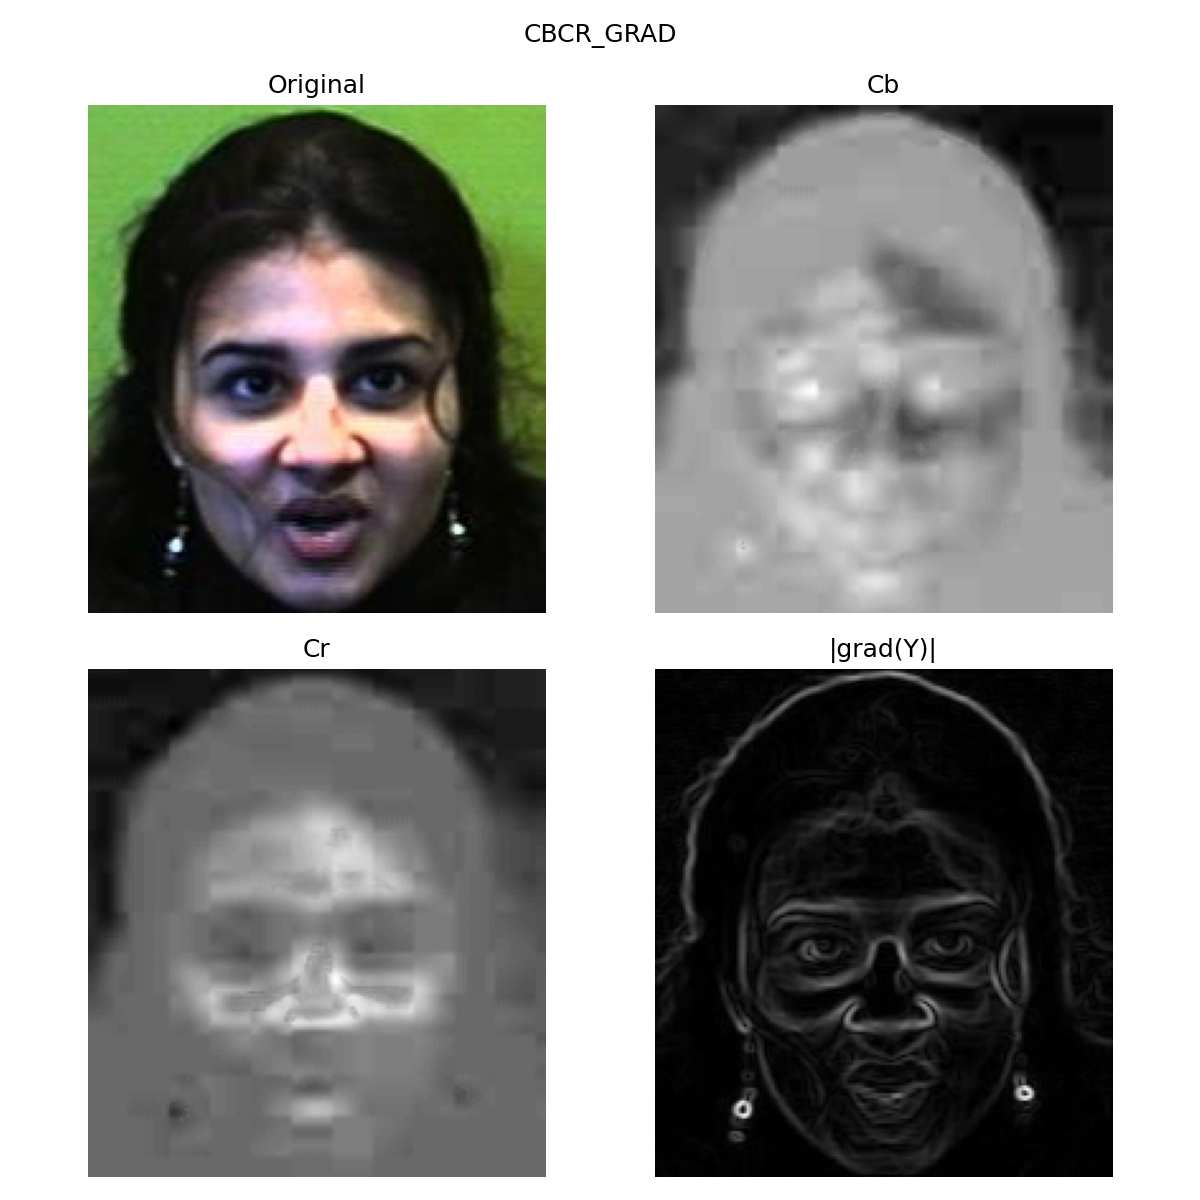
\includegraphics[width=0.95\columnwidth]{../../outputs/components/asamma.19/cbcr_grad/figure.png}
\caption{Visualisation de la caract\'eristique locale \texttt{cbcr\_grad} sur l'image \texttt{asamma.19.jpg} : image originale, \(Cb\), \(Cr\) et \(|\nabla Y|\).}
\label{fig:face_cbcr_grad}
\end{figure}

Les composantes \(Cb\) et \(Cr\) gardent une bonne coh\'erence sur les zones de peau, comme dans l'espace YCrCb, mais l'ajout de \(|\nabla Y|\) fait appara\^itre plus nettement les contours et transitions locales significatives : bord du visage, yeux, bouche, fronti\`eres entre la peau et les cheveux, ainsi qu'entre le visage et l'arri\`ere-plan. Par rapport \`a YCrCb seul, cette combinaison introduit donc une information de structure locale sans quitter une repr\'esentation compacte \`a trois dimensions.

Cette caract\'eristique est plus favorable \`a un mod\`ele bay\'esien de d\'etection peau / non-peau, car elle aide \`a mieux distinguer les r\'egions ambigu\"es o\`u la couleur seule ne suffit pas, en particulier sur les fronti\`eres et dans les zones partiellement ombr\'ees. Sa limite est que le gradient r\'eagit aussi aux ombres, \`a certaines textures et aux accessoires. En pratique, cela signifie que les exemples n\'egatifs utilis\'es pendant l'apprentissage doivent couvrir non seulement le fond, mais aussi les cheveux, les yeux et les zones sombres du visage, afin d'\'eviter qu'un contour marqu\'e soit confondu avec une zone de peau.

\subsubsection{\textbf{Modification du mod\`ele d'entra\^inement}}

Le script \texttt{Bayes\_Model\_Training.py} a \'et\'e adapt\'e pour exploiter \texttt{cbcr\_grad} comme espace d'observation par d\'efaut. L'interface accepte d\'esormais une ou plusieurs images d'apprentissage en argument positionnel, ce qui permet soit de conserver le cas simple \`a une seule image, soit d'agr\'eger des annotations provenant de plusieurs visages avant l'estimation du mod\`ele bay\'esien. L'argument \texttt{--test-image} reste optionnel et, s'il n'est pas fourni, la premi\`ere image d'apprentissage est utilis\'ee comme image de test.

L'extraction des caract\'eristiques est maintenant unifi\'ee avec le module \texttt{features.py}. Le descripteur \texttt{cbcr\_grad} utilis\'e pendant l'entra\^inement est donc exactement le m\^eme que celui visualis\'e dans la section pr\'ec\'edente, ce qui garantit la coh\'erence entre l'analyse exploratoire et la construction du mod\`ele probabiliste. Pour chaque pixel, le vecteur d'observation est form\'e par \((Cb, Cr, |\nabla Y|)\), c'est-\`a-dire deux composantes de chrominance et une mesure locale de contour.

Le flux d'annotation supervis\'ee a \'egalement \'et\'e \'etendu \`a plusieurs images. Chaque image est ouverte successivement, les r\'egions d'int\'er\^et annot\'ees \texttt{skin} et \texttt{non\_skin} sont converties en lots de pixels, puis toutes les annotations sont concat\'en\'ees dans une base d'apprentissage unique avant l'ajustement du classifieur. Les commandes manuelles restent inchang\'ees : \texttt{p} pour annoter la peau, \texttt{n} pour le non-peau, \texttt{r} pour r\'einitialiser la RoI courante et \texttt{q} pour passer \`a l'image suivante, ou terminer l'annotation lorsqu'il s'agit de la derni\`ere image. Enfin, les m\'etadonn\'ees sauvegard\'ees enregistrent d\'esormais la liste des images d'apprentissage utilis\'ees pour la corrida.

Pour le protocole recommand\'e dans ce rapport, nous sugg\'erons d'annoter \texttt{img/Essex\_Faces/94/asamma.19.jpg} comme image d'apprentissage, puis de tester le mod\`ele appris sur \texttt{img/Essex\_Faces/94/ajones.19.jpg}, \texttt{img/Essex\_Faces/94/asheal.18.jpg}
et \texttt{img/Essex\_Faces/96/acatsa.17.jpg}. Un jeu d'annotations raisonnable consiste \`a s\'electionner environ 5 \`a 8 RoI de peau et 5 \`a 8 RoI de non-peau, en veillant \`a inclure parmi les n\'egatifs le fond, les cheveux, les yeux, les sourcils et les zones d'ombre. Ce choix limite le risque que la composante de gradient favorise \`a tort des contours marqu\'es qui ne correspondent pas \`a la peau.

\subsubsection{\textbf{Résultats du modèle bayésien gaussien multidimensionnel}}

\begin{figure*}[!t]
\centering
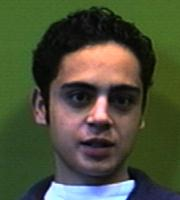
\includegraphics[width=0.24\textwidth]{../../img/Essex_Faces/94/ajones.19.jpg}\hfill
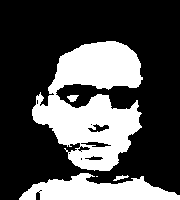
\includegraphics[width=0.24\textwidth]{../../outputs/bayes/ajones.19/cbcr_grad_qda_map/mask.png}\hfill
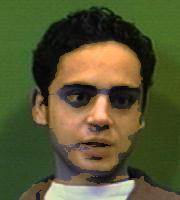
\includegraphics[width=0.24\textwidth]{../../outputs/bayes/ajones.19/cbcr_grad_qda_map/overlay.png}\hfill
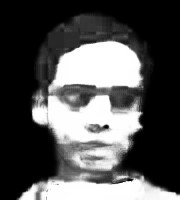
\includegraphics[width=0.24\textwidth]{../../outputs/bayes/ajones.19/cbcr_grad_qda_map/skin_probability.png}
\caption{Cas A -- \texttt{ajones.19.jpg}. De gauche \`a droite : image originale, masque binaire pr\'edit, superposition de la d\'etection sur l'image et carte de probabilit\'e de peau.}
\label{fig:bayes_case_a}
\end{figure*}

Le cas A constitue un premier quasi-succ\`es du mod\`ele appris sur \texttt{asamma.19}. Le masque binaire localise correctement une grande partie de la peau du visage et l'\textit{overlay} confirme que la r\'egion faciale principale est bien d\'etect\'ee. La carte de probabilit\'e reste \'elev\'ee sur les joues, le front et le menton, ce qui montre que le mod\`ele reconna\^it de mani\`ere coh\'erente les zones cutan\'ees dominantes. On observe toutefois des faux positifs sur une partie du v\^etement et autour de certaines transitions \`a fort contraste, ce qui indique que la s\'eparation peau / non-peau n'est pas encore compl\`ete.

\begin{figure*}[!t]
\centering
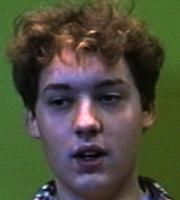
\includegraphics[width=0.24\textwidth]{../../img/Essex_Faces/94/asheal.18.jpg}\hfill
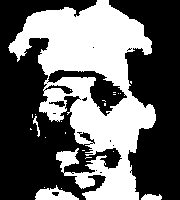
\includegraphics[width=0.24\textwidth]{../../outputs/bayes/asheal.18/cbcr_grad_qda_map/mask.png}\hfill
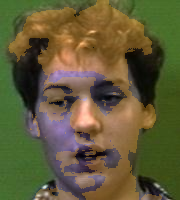
\includegraphics[width=0.24\textwidth]{../../outputs/bayes/asheal.18/cbcr_grad_qda_map/overlay.png}\hfill
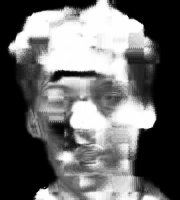
\includegraphics[width=0.24\textwidth]{../../outputs/bayes/asheal.18/cbcr_grad_qda_map/skin_probability.png}
\caption{Cas B -- \texttt{asheal.18.jpg}. De gauche \`a droite : image originale, masque binaire pr\'edit, superposition de la d\'etection sur l'image et carte de probabilit\'e de peau.}
\label{fig:bayes_case_b}
\end{figure*}

Le cas B pr\'esente lui aussi un r\'esultat globalement satisfaisant, avec une bonne d\'etection de la peau sur le visage et une structure g\'en\'erale assez proche de celle obtenue sur l'image d'apprentissage. Le masque et l'\textit{overlay} montrent cependant que les cheveux sont partiellement class\'es comme peau, en particulier dans les zones claires et tr\`es contrast\'ees. La carte de probabilit\'e confirme que le mod\`ele attribue localement une forte confiance \`a ces r\'egions, ce qui sugg\`ere un recouvrement partiel entre certaines signatures de chrominance / gradient du visage appris et celles des cheveux dans cette image.

\begin{figure*}[!t]
\centering
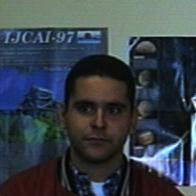
\includegraphics[width=0.24\textwidth]{../../img/Essex_Faces/96/acatsa.17.jpg}\hfill
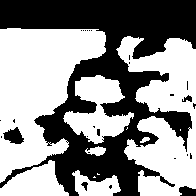
\includegraphics[width=0.24\textwidth]{../../outputs/bayes/acatsa.17/cbcr_grad_qda_map/mask.png}\hfill
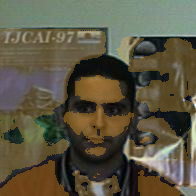
\includegraphics[width=0.24\textwidth]{../../outputs/bayes/acatsa.17/cbcr_grad_qda_map/overlay.png}\hfill
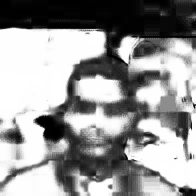
\includegraphics[width=0.24\textwidth]{../../outputs/bayes/acatsa.17/cbcr_grad_qda_map/skin_probability.png}
\caption{Cas C -- \texttt{acatsa.17.jpg}. De gauche \`a droite : image originale, masque binaire pr\'edit, superposition de la d\'etection sur l'image et carte de probabilit\'e de peau.}
\label{fig:bayes_case_c}
\end{figure*}

Le cas C est nettement moins convaincant. Le masque envahit une partie importante du fond et de plusieurs r\'egions non cutan\'ees, tandis que l'\textit{overlay} montre une segmentation trop \'etendue autour du visage. La carte de probabilit\'e attribue aussi des valeurs \'elev\'ees \`a des zones qui ne devraient pas \^etre interpr\'et\'ees comme de la peau. Le mod\`ele parvient encore \`a rep\'erer une partie du visage, mais il perd ici en sp\'ecificit\'e et confond plus largement la peau avec le d\'ecor et certains objets de l'image.

Les cas A et B peuvent donc \^etre consid\'er\'es comme des cas de quasi-r\'eussite. Dans les deux situations, le visage et la peau sont d\'etect\'es de mani\`ere visiblement meilleure que le fond g\'en\'eral, ce qui montre que le descripteur \texttt{cbcr\_grad} apporte une information utile. La combinaison de \(Cb\), \(Cr\) et \(|\nabla Y|\) pr\'eserve en effet une coh\'erence suffisante sur les zones principales de peau tout en exploitant une information locale de contour. Les faux positifs sur les v\^etements dans le cas A ou sur les cheveux dans le cas B n'annulent pas ce r\'esultat, mais ils r\'ev\`elent que la fronti\`ere statistique apprise entre peau et non-peau reste imparfaite.

Ces erreurs s'expliquent en grande partie par le protocole d'apprentissage lui-m\^eme. Le mod\`ele a \'et\'e appris \`a partir d'une seule image, \texttt{asamma.19}, ce qui lui donne une vision tr\`es limit\'ee de la variabilit\'e r\'eelle des apparences de peau et de non-peau. En outre, l'annotation manuelle n'a \'et\'e r\'ealis\'ee qu'une seule fois ; elle peut donc \^etre sensible \`a des RoI imparfaites, \`a un biais dans le choix des exemples et \`a une couverture incompl\`ete des cas n\'egatifs difficiles. Dans ce contexte, des r\'egions comme les cheveux clairs, les v\^etements ou certaines zones tr\`es contrast\'ees peuvent partager avec la peau des signatures locales proches en chrominance ou en contraste, et \texttt{cbcr\_grad}, bien qu'il am\'eliore la robustesse vis-\`a-vis de l'illumination, ne supprime pas totalement ce recouvrement statistique.

Le comportement du cas C permet de mieux comprendre cette limite. L'introduction de \texttt{cbcr\_grad} r\'eduit effectivement une partie de la sensibilit\'e \`a la luminance seule, mais elle n'\'elimine pas le probl\`eme de changement de domaine entre l'image d'apprentissage et une image de test tr\`es diff\'erente. Ici, le fond, le style photographique, le contraste global et la distribution locale des couleurs et des textures de \texttt{acatsa.17} s'\'ecartent davantage de ceux de \texttt{asamma.19}. Or le mod\`ele QDA apprend une distribution gaussienne corr\'el\'ee \`a partir des exemples annot\'es ; lorsqu'il n'a vu qu'une seule image d'entra\^inement, il g\'en\'eralise mal d\`es que l'apparence du nouveau cas s'\'eloigne trop des statistiques initiales. Autrement dit, \texttt{cbcr\_grad} aide \`a mieux repr\'esenter la peau, mais il reste d\'ependant des statistiques locales observ\'ees pendant l'apprentissage. Si le fond, les cheveux ou les objets du cas C pr\'esentent des combinaisons de \(Cb\), \(Cr\) et \(|\nabla Y|\) peu ou mal couvertes dans les annotations initiales, des faux positifs apparaissent malgr\'e l'enrichissement du descripteur.

En conclusion, ces r\'esultats montrent que \texttt{cbcr\_grad} constitue bien une am\'elioration par rapport \`a une repr\'esentation purement colorim\'etrique, car il combine l'information de peau et l'information de contour. N\'eanmoins, une seule image d'apprentissage et une seule it\'eration d'annotation restent insuffisantes pour obtenir une g\'en\'eralisation robuste sur des images plus vari\'ees. L'am\'elioration la plus naturelle ne serait donc pas d'abandonner ce descripteur, mais d'augmenter la diversit\'e des images d'apprentissage et de couvrir davantage de cas n\'egatifs difficiles pendant l'annotation.

\subsubsection{\textbf{Résultats du modèle bayésien gaussien naive}}

\begin{figure*}[!t]
\centering
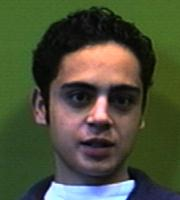
\includegraphics[width=0.24\textwidth]{../../img/Essex_Faces/94/ajones.19.jpg}\hfill
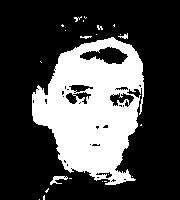
\includegraphics[width=0.24\textwidth]{../../outputs/bayes/ajones.19/cbcr_grad_gnb_map/mask.png}\hfill
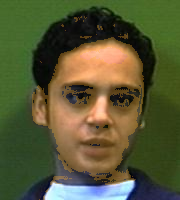
\includegraphics[width=0.24\textwidth]{../../outputs/bayes/ajones.19/cbcr_grad_gnb_map/overlay.png}\hfill
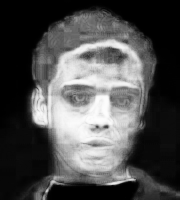
\includegraphics[width=0.24\textwidth]{../../outputs/bayes/ajones.19/cbcr_grad_gnb_map/skin_probability.png}
\caption{Cas A-na\"if -- \texttt{ajones.19.jpg}. De gauche \`a droite : image originale, masque binaire pr\'edit, superposition de la d\'etection sur l'image et carte de probabilit\'e de peau.}
\label{fig:bayes_naive_case_a}
\end{figure*}

Dans le cas A, le mod\`ele gaussien na\"if fournit une d\'etection qui reste coh\'erente sur l'essentiel du visage, tout en r\'eduisant certains faux positifs observ\'es pr\'ec\'edemment sur les v\^etements et autour de quelques bordures non faciales. Le masque est plus contenu, l'\textit{overlay} appara\^it plus propre sur les r\'egions non cutan\'ees, et la carte de probabilit\'e reste concentr\'ee sur les zones du visage les plus plausibles. L'explication la plus probable est que \texttt{GaussianNB} suppose une ind\'ependance entre les composantes observ\'ees \((Cb, Cr, |\nabla Y|)\), au lieu de mod\'eliser leur covariance compl\`ete comme QDA. Avec une seule image d'entra\^inement, cette hypoth\`ese plus simple peut rendre le mod\`ele moins sensible \`a des corr\'elations sp\'ecifiques et accidentelles apprises sur \texttt{asamma.19}, ce qui le rend ici plus conservateur hors de la r\'egion faciale principale.

\begin{figure*}[!t]
\centering
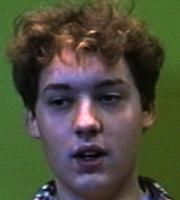
\includegraphics[width=0.24\textwidth]{../../img/Essex_Faces/94/asheal.18.jpg}\hfill
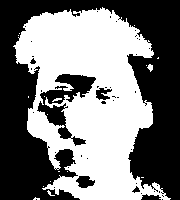
\includegraphics[width=0.24\textwidth]{../../outputs/bayes/asheal.18/cbcr_grad_gnb_map/mask.png}\hfill
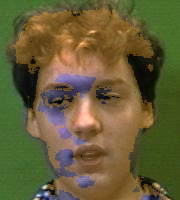
\includegraphics[width=0.24\textwidth]{../../outputs/bayes/asheal.18/cbcr_grad_gnb_map/overlay.png}\hfill
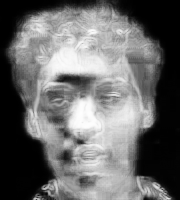
\includegraphics[width=0.24\textwidth]{../../outputs/bayes/asheal.18/cbcr_grad_gnb_map/skin_probability.png}
\caption{Cas B-na\"if -- \texttt{asheal.18.jpg}. De gauche \`a droite : image originale, masque binaire pr\'edit, superposition de la d\'etection sur l'image et carte de probabilit\'e de peau.}
\label{fig:bayes_naive_case_b}
\end{figure*}

Dans le cas B, le r\'esultat obtenu avec le mod\`ele na\"if reste globalement tr\`es proche de celui du mod\`ele gaussien multidimensionnel. La peau principale est toujours correctement d\'etect\'ee sur le visage, mais les faux positifs sur les cheveux demeurent du m\^eme ordre de grandeur. Cela sugg\`ere que, pour cette image, la difficult\'e ne provient pas d'abord de la mani\`ere de mod\'eliser les corr\'elations entre composantes, mais plut\^ot du fait que certaines zones de cheveux poss\`edent d\'ej\`a, au niveau m\^eme des caract\'eristiques locales \(Cb\), \(Cr\) et \(|\nabla Y|\), une signature assez proche de celle des zones de peau apprises. Dans un tel cas, passer d'une covariance compl\`ete \`a une hypoth\`ese d'ind\'ependance ne modifie pas fortement la d\'ecision finale.

\begin{figure*}[!t]
\centering
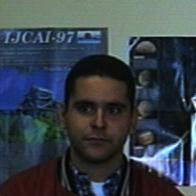
\includegraphics[width=0.24\textwidth]{../../img/Essex_Faces/96/acatsa.17.jpg}\hfill
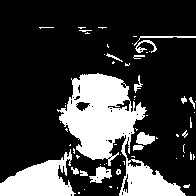
\includegraphics[width=0.24\textwidth]{../../outputs/bayes/acatsa.17/cbcr_grad_gnb_map/mask.png}\hfill
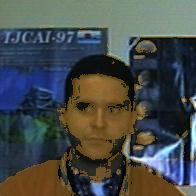
\includegraphics[width=0.24\textwidth]{../../outputs/bayes/acatsa.17/cbcr_grad_gnb_map/overlay.png}\hfill
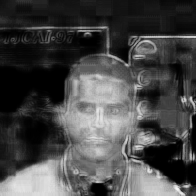
\includegraphics[width=0.24\textwidth]{../../outputs/bayes/acatsa.17/cbcr_grad_gnb_map/skin_probability.png}
\caption{Cas C-na\"if -- \texttt{acatsa.17.jpg}. De gauche \`a droite : image originale, masque binaire pr\'edit, superposition de la d\'etection sur l'image et carte de probabilit\'e de peau.}
\label{fig:bayes_naive_case_c}
\end{figure*}

Dans le cas C, le mod\`ele na\"if donne un r\'esultat nettement meilleur que le mod\`ele gaussien multidimensionnel, en particulier parce que le fond n'est plus massivement interpr\'et\'e comme de la peau. Le masque est plus resserr\'e autour du visage, l'\textit{overlay} laisse davantage le d\'ecor intact, et la carte de probabilit\'e ne diffuse plus aussi fortement sur l'arri\`ere-plan. Cette am\'elioration est remarquable car l'image originale pr\'esente justement un fond tr\`es diff\'erent de celui de \texttt{asamma.19}, qui a servi \`a l'entra\^inement. Le descripteur \texttt{cbcr\_grad} aide toujours \`a r\'eduire la sensibilit\'e \`a la luminance seule, mais ici l'effet favorable vient surtout du fait que le mod\`ele na\"if g\'en\'eralise mieux sous changement de domaine : en n'ajustant pas les corr\'elations entre composantes \`a partir d'une image unique, il \'evite de sur-sp\'ecialiser sa fronti\`ere de d\'ecision aux statistiques particuli\`eres du cas d'apprentissage. L'hypoth\`ese d'ind\'ependance joue alors comme une forme de r\'egularisation implicite.

Il est important de pr\'eciser que le caract\`ere ``na\"if'' du mod\`ele ne signifie pas une absence de corr\'elation entre les pixels de l'image. L'hypoth\`ese porte sur l'ind\'ependance conditionnelle des composantes du vecteur d'observation, c'est-\`a-dire ici \(Cb\), \(Cr\) et \(|\nabla Y|\), \`a l'int\'erieur d'une m\^eme classe. Le mod\`ele gaussien multidimensionnel, au contraire, prend explicitement en compte les corr\'elations entre ces composantes.

En comparant les deux approches, le mod\`ele gaussien na\"if pr\'esente plusieurs avantages : il est plus simple, il semble moins sensible \`a un surapprentissage de corr\'elations accidentelles, et il se montre plus robuste dans certains cas de changement de domaine comme \texttt{acatsa.17}. Il peut aussi r\'eduire certains faux positifs, comme sur les v\^etements dans le cas A. En revanche, il perd l'information sur les corr\'elations r\'eelles entre \(Cb\), \(Cr\) et \(|\nabla Y|\), ce qui peut limiter sa pr\'ecision lorsque ces d\'ependances sont effectivement discriminantes. On en conclut qu'aucun des deux mod\`eles ne domine syst\'ematiquement l'autre : avec une seule image d'apprentissage, le mod\`ele na\"if peut mieux g\'en\'eraliser, tandis que le mod\`ele gaussien multidimensionnel peut mieux exploiter la structure des donn\'ees lorsque les statistiques de test restent proches de celles observ\'ees \`a l'entra\^inement.
